\section{Introduction}
\begin{figure*}[t]
    \centering
        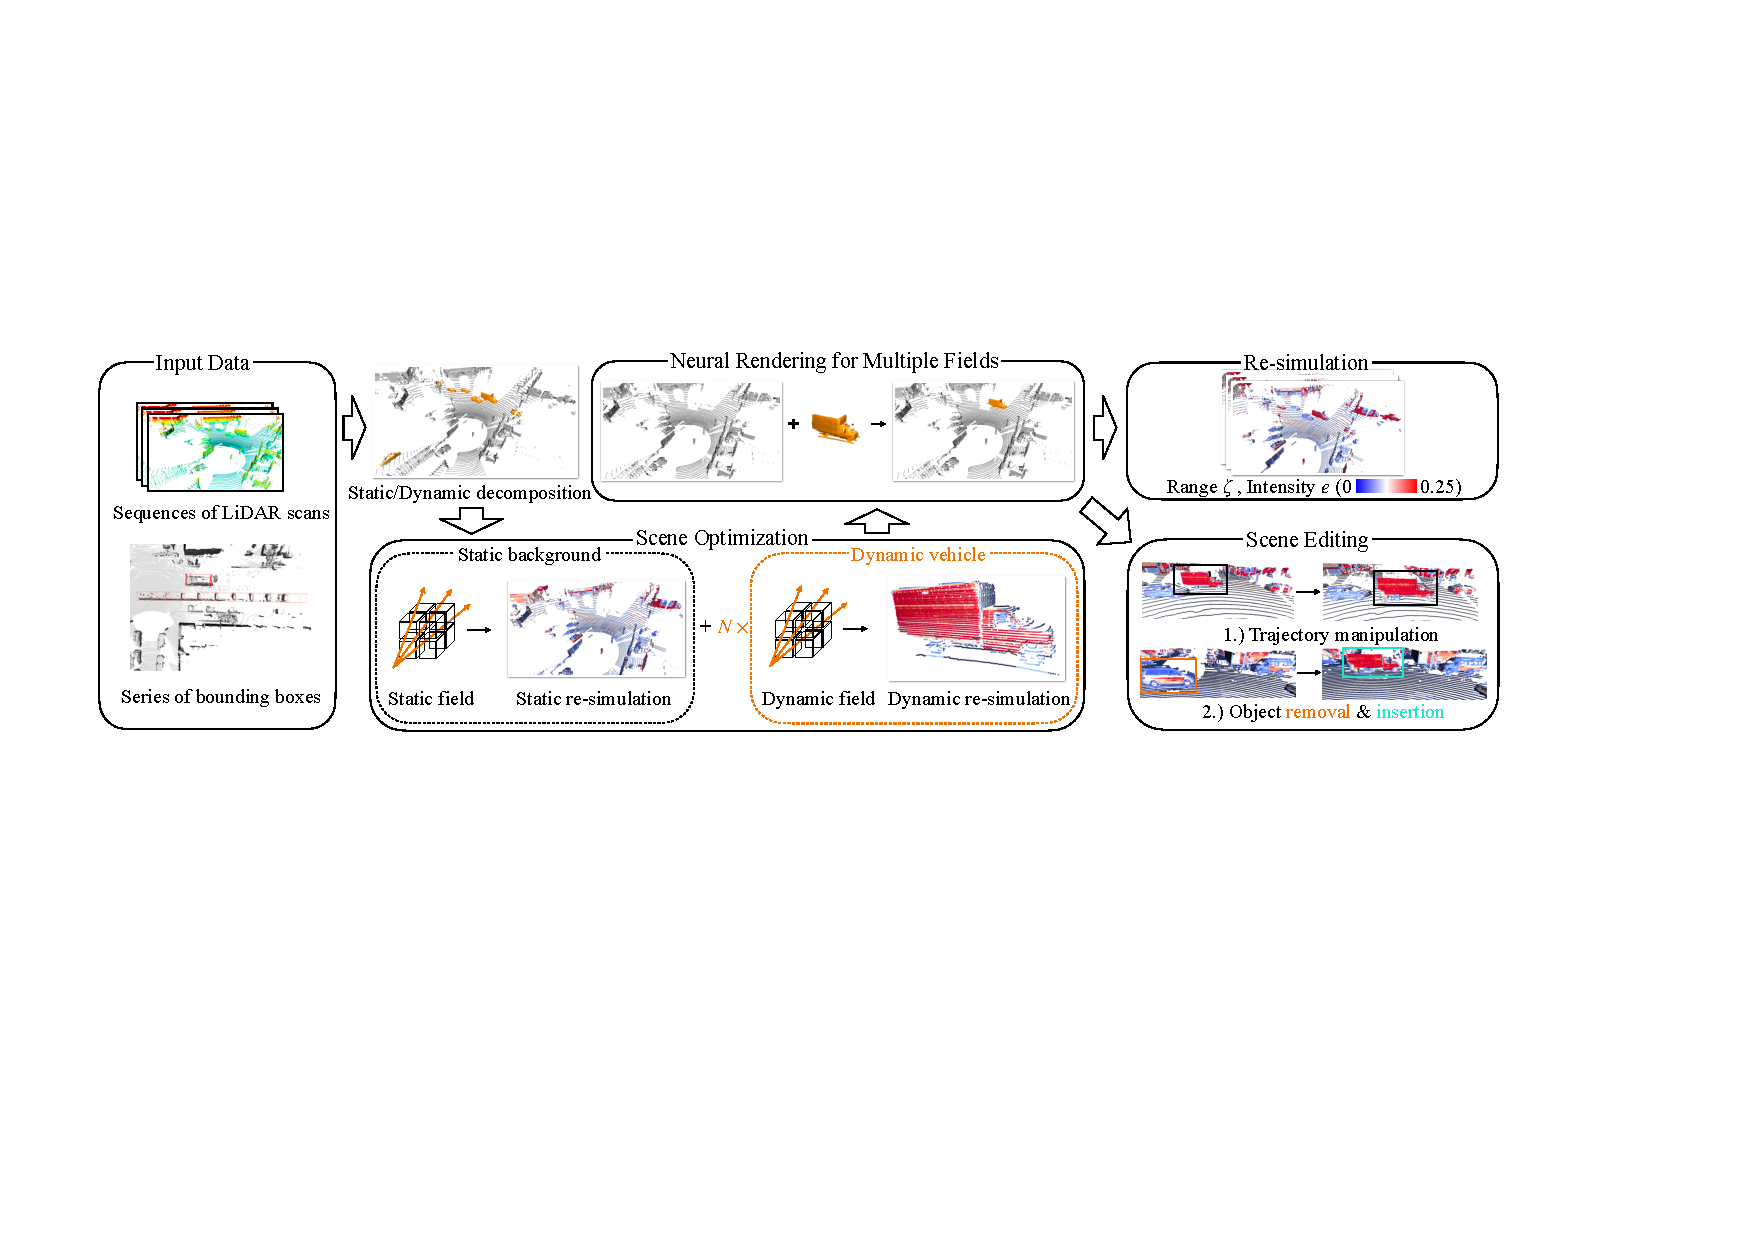
\includegraphics[width=1.0\textwidth]{Figures/overview.pdf}
        \caption{
        Overview of \dynfl. Our method takes LiDAR scans and tracked bounding boxes of dynamic vehicles as input. \dynfl first decomposes the scene into a static background and $N$ dynamic vehicles, each modelled using a dedicated neural field. These neural fields are then composed to re-simulate LiDAR scans in dynamic scenes. Our composition technique supports various scene edits, including altering object trajectories, removing and adding reconstructed neural assets between scenes.
    }
    \label{fig:main}
\end{figure*}

We introduce a neural representation for the purpose of reconstructing and manipulating LiDAR scans of dynamic driving scenes. 
Counterfactual re-simulation is an emerging application in the realm of autonomous driving, offering a unique approach to examining "what if" scenarios. This method involves creating a reconstruction of a real-world event, termed as \textit{digital twin} and then applying various modifications to it. These could include altering the environmental conditions, changing the action of some agent, or introducing additional scene elements. Analyzing the outcomes of these edited scenarios provides insights into the functioning of the perception system, moreover they can be used to obtain training data for rare situations.

The essence of counterfactual re-simulation is the capability to authentically recreate variations of the original, factual observation. We address this challenge in the context of LiDAR on autonomous vehicles (AV). Existing approaches to LiDAR re-simulation have important limitations. Conventional simulators such as CARLA~\cite{dosovitskiy2017carla} and NVIDIA DRIVE Sim are capable of modeling LiDAR sensors. However, their reliance on manually designed 3D simulation assets requires significant human effort. LiDARsim~\cite{manivasagam2020lidarsim} aims to remedy this by reconstructing vehicles and scenes from real measurements. While producing encouraging results, its two-stage LiDAR modeling lacks realism, particularly in terms of physical effects like multi-returns and reflected intensity, which were shown 
 to matter for downstream processing~\cite{guillard2022learning}. Following NeRF's~\cite{mildenhall2020nerf} success in camera view synthesis, some works have applied neural fields for LiDAR modeling~\cite{Huang2023nfl, tao2023lidar, zhang2023nerf}. In particular, Neural LiDAR Fields (NFL)\cite{Huang2023nfl} developed a physically inspired LiDAR volumetric rendering scheme that accounts for two-way transmittance and beam width, allowing faithful recovery of secondary returns, intensity, and ray drops. These models are, however, limited to static scenes that do not change while multiple input views are scanned, and are thus of limited use for re-simulation in the presence of moving traffic. Recently, UniSim~\cite{yang2023unisim} followed Neural Scene Graph~\cite{Ost_2021_CVPR} in modeling road scenes as sets of movable NeRF instances on top of a static background. UniSim introduced a unified synthesis approach for camera and LiDAR sensors, but ignored physical sensor properties like two-way transmittance and beam width~\cite{Huang2023nfl}.

We present \dynfl, a novel approach for re-simulating LiDAR views of driving scenarios. Our method builds upon a neural SDF that enables an accurate representation of scene geometry, while at the same time enforcing physical accuracy by modeling two-way transmittance, like NFL~\cite{Huang2023nfl}. 
% Our method builds upon UniSim's SDF representation and scene decomposition, but enhances the physical accuracy by incorporating two-way transmittance modeling, as introduced in NFL.
%
Our primary contribution is a method for compositing neural fields that accurately integrates LiDAR measurements from individual fields representing different scene assets. With the help of a ray drop test, we effectively manage occlusions and transparent surfaces. This not only ensures physical accuracy, but also facilitates the inclusion of assets reconstructed from a variety of static and dynamic scenes, thereby enhancing control over the simulated content. Our method bridges the gap between the physical fidelity of the re-simulation and flexible editing of dynamic scenes.
%
We validate \dynfl with both synthetic and real-world data, focusing on three key areas: \textit{(i)} high-quality view synthesis, \textit{(ii)} perceptual fidelity, and \textit{(iii)} asset manipulation. We find that our approach outperforms baseline models \wrt both range and intensity. Its synthetic outputs also show higher agreement with real scans in terms of object detection and segmentation. Furthermore, \dynfl enables not only removal, duplication and repositioning of assets within the same scene, but also the inclusion of assets reconstructed in other scenes, paving the way for new applications.


% In the rapidly evolving field of computer vision, novel view synthesis has become a groundbreaking technique, especially in the realm of image-based rendering. Pioneered by technologies like NeRF~\cite{mildenhall2020nerf}, it allows for the creation of photo-realistic views from a given set of data. However, the application of these principles to LiDAR data, which inherently deals with point clouds, introduces a complex set of challenges and opportunities that are distinct from traditional image-based approaches.

% Historically, methods like LiDARsim~\cite{manivasagam2020lidarsim} have paved the way for such advancements, yet they exhibit limitations. Specifically, LiDARsim operates by first extracting an explicit scene representation and then performing ray-surfel casting to synthesize LiDAR scans. This approach, while innovative, is susceptible to inaccuracies due to point cloud noise and typically results in lower reconstruction quality. This limitation leads to a significant domain gap when compared to ground truth LiDAR scans. Our previous work, Neural Lidar Fields (NFL)~\cite{Huang2023nfl}, marked a substantial improvement in modeling LiDAR scenes with neural fields and incorporating the physical characteristics of LiDAR beams. Despite its state-of-the-art performance in geometry reconstruction, NFL was limited to static scenes and did not address the complexities of dynamic environments.

% In dynamic scenarios, particularly in automotive or robotics contexts, capturing the constant motion of elements like vehicles and pedestrians is crucial. Our work seeks to bridge this gap by extending the principles of NFL to dynamic settings. Prior approaches that tackle the dynamic scenes, such as LiDARsim~\cite{manivasagam2020lidarsim}, have adopted a reconstruct-then-simulate process, resulting in inferior geometric fidelity. Meanwhile, other neural-fields-based explorations like Neural Scene Graph~\cite{Ost_2021_CVPR} and UniSim~\cite{yang2023unisim} focus on image-based rendering or sensor fusion, neglecting LiDAR-specific attributes.

% In this context, our work contributes in several ways:
% \textbf{1.)} Improved Geometry Quality: We adopt a Signed Distance Function (SDF)-based volume rendering approach, specifically tailored to the active sensor characteristics of LiDAR beam. This method acknowledges and leverages the intricacies of how LiDAR sensors capture data, resulting in reconstructions of higher fidelity and geometric accuracy.
% \textbf{2.)} Innovative Neural Fields Composition: Our methodology introduces a novel technique for the composition of multiple neural fields. This approach significantly enhances the rendering process, allowing for seamless integration and higher-quality synthesis of dynamic views.

% Our paper delves into the technicalities of Dynamic Neural LiDAR Fields, elaborating on the methods and innovations that enable the synthesis of dynamic views from LiDAR data. We present extensive experimental results that showcase the effectiveness of our approach in dynamic environments, illustrating how our contributions extend the applicability of neural LiDAR fields. Through this work, we provide a valuable resource for researchers in computer vision, contributing to the broader discourse on LiDAR novel view synthesis for dynamic scenes.

